\section{Convexity, Lipschitzness, and Smoothness}
\frame{\tableofcontents[currentsection, hideothersubsections]}

\begin{frame}
\frametitle{Convexity: Convex sets}

\begin{figure}
    \centering
    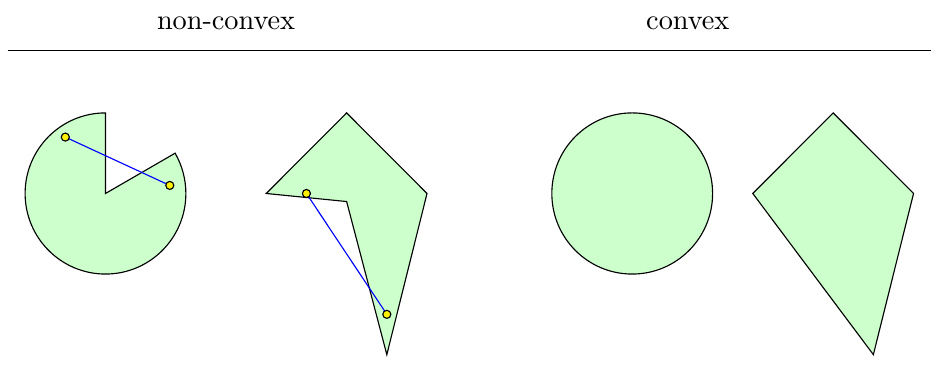
\includegraphics[scale=0.35]{cvx_noncvx}
\end{figure}

\begin{figure}
    \centering
    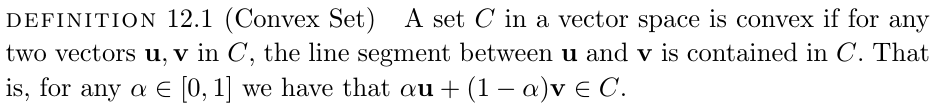
\includegraphics[scale=0.4]{cvx_set}
\end{figure}

\end{frame}

\begin{frame}
\frametitle{Convexity: Convex functions}

\begin{figure}
    \centering
    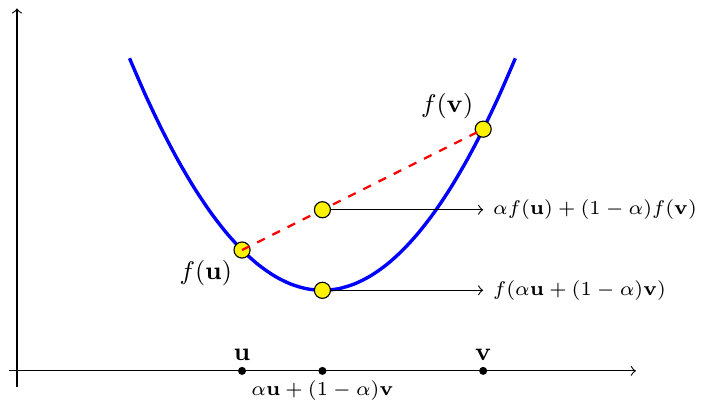
\includegraphics[scale=0.35]{cvx_fn}
\end{figure}

\begin{figure}
    \centering
    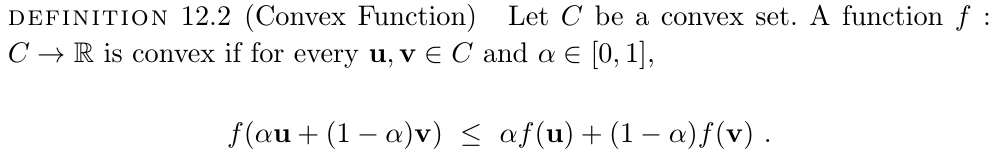
\includegraphics[scale=0.4]{cvx_fn_def}
\end{figure}

\end{frame}

\begin{frame}
\frametitle{Convexity: Convex functions}

Properties:
\begin{itemize}
    \item  every local minimum is also a global minimum
    \item  for every $\mathbf{w}$ we can construct a tangent to $f$
    at $\mathbf{w}$ that lies below $f$ everywhere.
    If f is differentiable, this tangent is the linear function
    % $l(u) = f(w) + h∇f (w), u − wi$
\end{itemize}

\begin{figure}
    \centering
    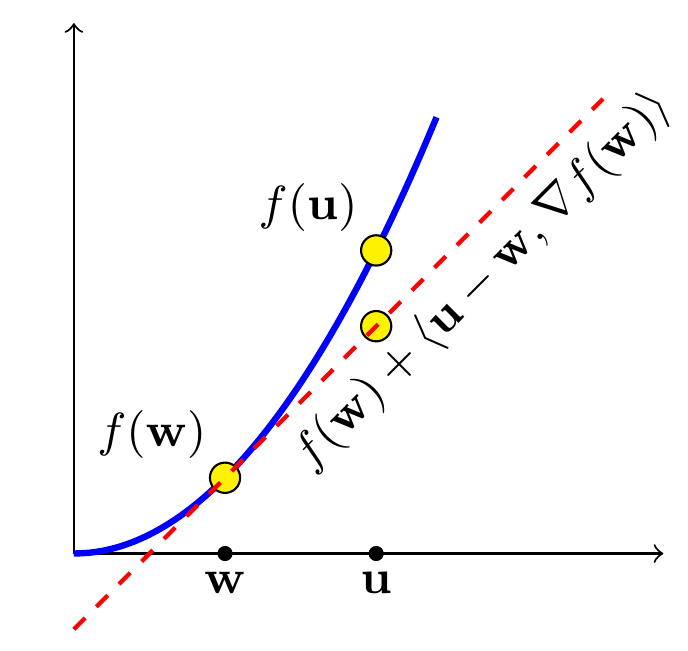
\includegraphics[scale=0.25]{cvx_fn_tangent}
\end{figure}

\end{frame}

\begin{frame}
\frametitle{Convexity: Convex functions}

\begin{figure}
    \centering
    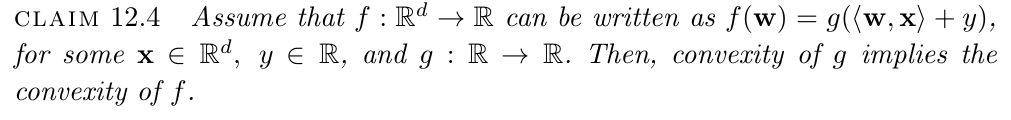
\includegraphics[scale=0.4]{claim_12_4}
\end{figure}

\begin{figure}
    \centering
    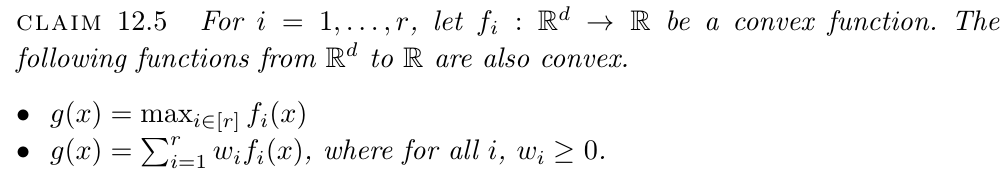
\includegraphics[scale=0.4]{claim_12_5}
\end{figure}

\end{frame}


\begin{frame}
\frametitle{Lipschitzness}
\begin{figure}
    \centering
    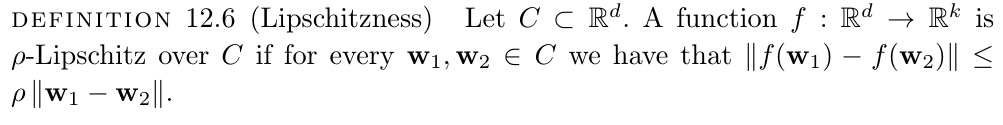
\includegraphics[scale=0.4]{def_12_6}
\end{figure}

\begin{itemize}
    \item a Lipschitz function cannot change too fast
    \item if the derivative of $f$ is everywhere bounded (in absolute value) by $\rho$,
        then the function is $\rho$-Lipschitz.
    \item composition of Lipschitz functions preserves Lipschitzness.
\end{itemize}

\end{frame}


\begin{frame}
\frametitle{Smoothness}
\begin{figure}
    \centering
    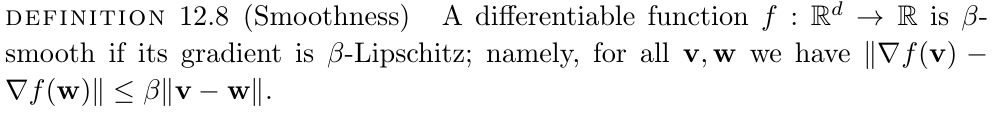
\includegraphics[scale=0.4]{def_12_8}
\end{figure}

\begin{itemize}
    \item when a function is both convex and smooth,\\
        we have both upper and lower bounds on the difference between
        the function and its first order approximation.
    \item a composition of a smooth scalar function over a linear function preserves smoothness.
\end{itemize}

\end{frame}
